\section{BPX Type: Model ('M')}

\subsection{Overview}
The Model BPX uses 'M' as the type byte of BPX Main Header. This type provides optimized and efficient mesh storage for 3D rendering APIs.
\newline
Below is a table describing the different sections to be expected in a BPXM:
\bpxsectiontable
{
    VertexArray & 2 & Yes & No \\
    IndexArray & 3 & No & No \\
    BoneArray & 4 & No & Yes \\
    FrameArray & 5 & No & Yes \\
    AnimationArray & 6 & No & Yes \\
    Strings & 255 & No & Yes \\
}

\subsection{TypeExt}
Contains general information about the 3D model file.
\bpxfieldtable
{
    ShaderHash & Unsigned & 64 & Hash of shader package virtual path \\
    SymbolName & Unsigned & 32 & Name of vertex format symbol in the shader package \\
    Reserved & Unsigned & 32 & Blank, always 0 \\
}
\begin{center}
    \begin{bytefield}[bitwidth=1.2em]{32}
        \bitheader{0-31} \\
        \begin{rightwordgroup}{128 bits}
            \bitbox{32}{ShaderHash} \\
            \bitbox{32}{ShaderHash} \\
            \bitbox{32}{SymbolName} \\
            \bitbox{32}{Reserved}
        \end{rightwordgroup}
    \end{bytefield}
\end{center}

\subsubsection{ShaderHash}
The hash of the virtual path of the shader package containing the vertex format of this model.

\subsubsection{SymbolName}
The symbol name of the vertex format to locate in the shader package identified by the ShaderHash field.

\subsection{VertexArray}
This section contains a header followed by an array of vertex data structure. The size of each vertex structure should be equal to the field VertexSize in the VertexFormat section.\newline
The header data structure is described in the following table:
\bpxfieldtable
{
    MaterialHash & Unsigned & 64 & Hash of material \\
    VertexCount & Unsigned & 32 & Total number of vertices \\
    IndexArray & Unsigned & 32 & Index array section index \\
    Reserved & Unsigned & 32 & Blank, always 0 \\
}
\begin{center}
    \begin{bytefield}[bitwidth=0.73em]{64}
        \bitheader{0-63} \\
        \bitbox{64}{MaterialHash} \\
		\bitbox{32}{VertexCount} & \bitbox{32}{IndexArray}
    \end{bytefield}
\end{center}

\subsubsection{MaterialHash}
The hash of the virtual path of the material asset to be applied as default.

\subsubsection{VertexCount}
The amount of vertex structures to read after this header.\newline
\textbf{Note that all modern hardware supports triangles as only primitive, so the vertex count should be a multiple of 3.}

\subsubsection{IndexArray}
This field is an index in the section header table to an IndexArray that should be used alongside this VertexArray.\newline
A value of $0$ means that no IndexArray is associated to that VertexArray.

\subsubsection{Total array size}
The total size in bytes of the vertex array to use as pre-allocation buffer size when loading this model can be calculated as follows:
\begin{equation}
    SA = S \times V
\end{equation}
where $SA$ is the total size of the vertex array, $S$ the size of a single vertex structure as given in the VertexFormat asset and $V$ the number of vertices in the array given by the VertexCount field.\newline
To avoid storing an additional 64 bits field in the header of the VertexArray section, this size $SA$ is left to be calculated by the implementing application.

\subsection{IndexArray}
The index array section allows to ommit certain vertices and figure out these vertices at runtime. Instead of writing all vertices for a given model requiring more space to store them, we only store unique vertices, and duplicates are just resolved by matching a vertex index from this section to an actual vertex structure, \textbf{this allows saving of storage space and RAM}.\newline
This section contains a header describing the amount of indices to be found in the array, and an array of 32 bits unsigned integers, each representing the index of a vertex in a given vertex array.\newline
Below is a table describing the data structure to expect as header for an IndexArray section:
\bpxfieldtable
{
    IndexCount & Unsigned & 32 & Total number of indices \\
}

\subsubsection{IndexCount}
The number of indices expected to be read from the array below this header.

\subsection{BoneArray}
This section contains a header followed by an array of data structures representing each bone in a skeletal mesh.\newline
Below is a description of the header to find before bone data in this section:
\bpxfieldtable
{
    BoneCount & Unsigned & 16 & Total number of bones \\
}

Each bone in the array following the header is represented by the following data structure:
\bpxfieldtable
{
    Head & 3D float vector & 96 & Initial position of bone head \\
    Tail & 3D float vector & 96 & Initial position of bone tail \\
    Name & Unsigned & 32 & Pointer in the Strings section \\
}
\begin{center}
    \begin{bytefield}[bitwidth=1.1em]{32}
        \bitheader{0-31} \\
        \bitbox{32}{Head [3]} \\
        \bitbox{32}{Tail [3]} \\
        \bitbox{32}{Name}
    \end{bytefield}
\end{center}

\subsubsection{BoneCount}
Number of bones to expect in the bone array following the header. This number should belong to the interval $[1, 1024]$.

\subsection{Analysis on theoretical bone limit}
We can give an estimation that the human skeleton can contain up to 400 bones. Of course most models do not include as many bones in order to reduce GPU/CPU load.
\begin{itemize}
    \item OpenGL, Vulkan and Metal maximum UBO/function constants storage size available to a shader is usually 64Kb or 65536 bytes
    \item On the official MSDN page \cite{MSDNConstantBuffers} for DirectX the maximum constant buffer size available to a shader is $4096 constants \times 4 \times 32 bits = 4096 constants \times 16 bytes = 65536 bytes$
\end{itemize}
UBO, function constants and constant buffer refers to means of variable synchronisation between CPU accessible memory and GPU accessible memory. Vulkan is a special case as it actually supports faster memory called Push Constants, however these constants usually max out at 256-512 bytes which is impracticable for storing bone transforms. Push constants are typically used to exchange important transformation matrices such as model, view or projection.
The size of a transformation matrix in 3D space expressed in homogeneous coordinate system \cite{HomogeneousCoordinates} is $32 bits (float) \times 4 \times 4 (4\times4 matrix) = 16 \times 32 bits = 512 bits = 64 bytes$.\newline
So, assuming the lowest size for storing bones in VRAM for GPU processing is $65536$ we can theoretically store up to $1024$ matrices, assuming each bone matrix represents 3D space transformations in homogeneous coordinate system ($\frac{65536}{64} = 1024$).\newline
Which means in order to \textbf{keep compatibility} with as many platforms/rendering apis as possible, also taking into account byte indexing, we should store the bone count as a 16 bits integer.

\subsubsection{Head}
Initial head position for that specific bone.

\subsubsection{Tail}
Initial tail position for that specific bone.

\subsubsection{Name}
Bone name as a pointer to a null terminated string in the strings section.

\subsection{FrameArray}
This section contains a header followed by an array of data structures each representing the new transform for a combination of a bone and frame.\newline
The array should be organized as the following diagram describes:
\begin{figure}[h!]
    \centering
    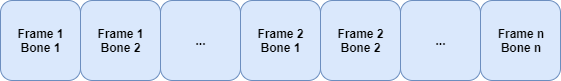
\includegraphics[scale=0.7]{Types/FrameArray_Diagram.png}
    \label{fig:FrameArray_Diagram}
    \caption{Diagram for organizing frame array}
\end{figure}
\newline
A single animation in a 3D model is usualy a set of actions. For example, consider the following set of actions on a 3D human based model:
\begin{itemize}
    \item move left leg
    \item move right leg
    \item move left arm
    \item move right arm
\end{itemize}
This set of actions could be grouped together in one animation named walking or running.\newline
We call total animation time the total time needed to express all animations for a single 3D model.

\subsubsection{Design decision}
The majority of mainstream formats represent animated models using key frames. That is, storing only determinant changes in the model and interpolating intermediate frames at runtime (either when loading the file or while rendering). In BPX type M, each frame is stored in the file to allow for any interpolation method. That is, the interpolation, if there is any, is defined by the exporting tool of that model. The engine runtime does not have to provide any interpolation function for BPX type M.\newline
This change grants the \textbf{flexibility} of using any interpolation function, even user defined.

\subsubsection{Analysis on theoretical required storage size}
We assume the total size required to store the full FrameArray is given by the following formula:
\begin{equation}
    F \times B \times B_s
\end{equation}
where $F$ is the total amount of frames, $B$ the number of bone updates per frame and $B_s$ the size of a single bone update structure.\newline
We previously indicated that a bone update is determined by a transformation matrix in homogeneous coordinate space \cite{HomogeneousCoordinates}, that means it is exactly $512bits$ or $64bytes$.\newline
Of course in a real application, it is very unlikely to have every frame in the timeline requiring update on every bone.
\vspace{12pt}
\newline\textbf{Worst case scenario}\newline
We assume the total animation time won't exceed $4$ minutes.\newline
We showed earlier that the theoretical maximum bone limit is $1024$.\newline
For the frame rate we choose $60$, that means each second, $60$ frames in this FrameArray have to be rendered.\newline
The total amount of frames to store is $60 \times 4 \times 60 = 14400frames$.\newline
The total size required to save a model assuming each frame requires dependency over exactly all bones is $14400 \times 1024 \times 512 = 7549747200bits = 943718400bytes$. That is approximately $944Mb$.
\vspace{12pt}
\newline\textbf{Average case scenario}\newline
Of course having $1024$ bones in one model is unlikely to happen. This is why we want to have an average estimation on the size required to store the FrameArray section.\newline
On average, the amount of bones per animated model won't exceed $50$ bones.\newline
On average, each frame will update at most $10$ bones.\newline
On average, the frame rate of a 3D model animation will be $30FPS$.\newline
On average, the total animation time won't exceed $2$ minutes.\newline
The total amount of frames to store is $30 \times 2 \times 60 = 3600frames$.\newline
The total size required to save the FrameArray of a model assuming each frame requires dependency over exactly all bones is $3600 \times 10 \times 512 = 18432000bits = 2304000bytes$. That is approximately $2Mb$.
\vspace{12pt}
\newline
In conclusion the FrameArray section \textbf{should be compressed} to reduce the storage space consumed by a single model asset on disk. When loading the model in RAM one might consider adding some compression or supporting a lower limit than $1024$ bones.

\subsubsection{Bone transform}
Each bone transformation in the FrameArray section is represented by the following structure:
\bpxfieldtable
{
    Rotation & 4D float vector & 128 & Target bone rotation as a quaternion \\
    Position & 3D float vector & 96 & Target bone position \\
    Scale & 3D float vector & 96 & Target bone scale \\
    BoneId & Unsigned & 32 & Index of affected bone \\
}
\begin{center}
    \begin{bytefield}[bitwidth=1.1em]{32}
        \bitheader{0-31} \\
        \bitbox{32}{Rotation [4]} \\
        \bitbox{32}{Position [3]} \\
        \bitbox{32}{Scale [3]} \\
        \bitbox{32}{BoneId}
    \end{bytefield}
\end{center}

\subsection{Strings}
The strings section contains a list of null-terminated strings to be referenced by start offset from other sections (see \ref{ssec:Strings}).